\documentclass[12pt, a4paper]{article}
\usepackage[UTF8]{ctex}
\usepackage{amsmath}
\usepackage{amssymb}
\usepackage{amsthm}
\usepackage{geometry}
\usepackage{enumitem}
\usepackage{indentfirst}
\usepackage{caption}
\usepackage{fancyhdr}
\usepackage{booktabs}
\usepackage{titlesec}
\usepackage{draftwatermark}%水印
\usepackage{graphicx} % 导入图像的宏包、单图
% 页面布局设置
\geometry{top=2.54cm, bottom=2.54cm, left=3.18cm, right=3.18cm}

\SetWatermarkText{B站：布加拉提}
\SetWatermarkScale{0.4}

% 行距设置
\linespread{1.5}

% 段落设置
\setlength{\parindent}{2em}
\setlength{\parskip}{0.5em}

% 节标题格式设置
\titleformat{\section}{\normalfont\Large\bfseries}{第\chinese{section}章、}{1em}{}
\titlespacing{\section}{0pt}{2.5ex plus 1ex minus .2ex}{1.3ex plus .2ex}

% 定理环境设置
\newtheoremstyle{solution}
{}
{}
{}
{}
{\bfseries}
{、}
{1em}
{}
\theoremstyle{solution}
\newtheorem{sol}{解}

% 页眉页脚设置
\pagestyle{fancy}
\fancyhf{}
\fancyhead[C]{b站布加拉提整理（回忆版）b站甘茶w独家讲解}
\fancyfoot[C]{\thepage}

\rfoot{整理人：八方\\资源提供：考研乔瑟夫}
\lhead{
\includegraphics[width=0.06\linewidth]{p1.png}}
\rhead{
\includegraphics[width=0.06\linewidth]{p2.png}}
\renewcommand{\headrulewidth}{0.4pt}
\renewcommand{\footrulewidth}{0.4pt}

\begin{document}

\begin{center}
\Large\textbf{2013哈工大硕士考试试题：805物理光学}
\end{center}





\section*{一、填空题（20分）}
\begin{enumerate}
    \item \_\_\_\_\_。
    \item \_\_\_\_\_称为波阵面。
    \item 产生干涉的条件是光波的\_\_\_\_\_。
    \item 平面波的复振幅数学表达式为\_\_\_\_\_，其物理含义是\_\_\_\_\_。
    \item 根据光的偏振特性，线偏振光（振动方向与入射面夹角不是0度和90度）在光密介质与光疏介质的界面上发生全反射时，反射光是\_\_\_\_\_。若线偏振光入射到金属表面时，反射光是\_\_\_\_\_，自然光从光密介质以布儒斯特角入射到光密介质时，反射光是\_\_\_\_\_，折射光是\_\_\_\_\_。
    \item 相位$\delta $与光程差$L$的关系为\_\_\_\_\_，采用光程概念的好处是\_\_\_\_\_。
    \item 波动过程的基本特征可用\_\_\_\_\_，\_\_\_\_\_和\_\_\_\_\_来描述。
    \item 点光源发出的光波在晶体中传播时，实际波面是\_\_\_\_\_，法线面是\_\_\_\_\_。
    \item 根据波动衍射成像理论，理想光学成像系统对点物在它像面上所成的像是\_\_\_\_\_图样。
\end{enumerate}
\section*{二、名词解释（27分）}
\begin{enumerate}
    \item 准单色光
    \item 群速度
    \item 艾里斑
    \item 巴比涅原理
    \item 半波损失
    \item 磁致旋光效应
    \item 色散
    \item 波片
    \item 双折射
\end{enumerate}
\section*{三、选择题（19分）}
\begin{enumerate}
    \item 直径为$1mm$的圆形光源，若波长为$0.5um$，在距光源$1m$的地方，其横向相干宽度为\_\_\_\_\_。\\(A)$0.3mm$\quad (B)$0.7mm$\quad (C)$0.51mm$\quad (D)$0.61mm$
    \item 若3个同频同振动方向的光波在某点$p$叠加，3个波依次相位差为$\pi/3$，振幅同为$A_0$，则$p$点的合振幅为\_\_\_\_\_，光强为\_\_\_\_\_。\\(A)$3A_0$\quad (B)$2A_0$\quad (C)$4A_0^2$\quad (D)$9A_0^2$
    \item 某激光的频宽为$\Delta \nu =5\times10^{14}HZ$,则该激光的波列长度为\_\_\_\_\_。\\(A)$600nm$\quad (B)$300nm$\quad (C)$200nm$\quad (D)$800nm$
    \item 在迈克尔逊干涉仪的两条光路中，分别垂直光路放置折射率为$n_1,n_2$，厚度$h$的透明介质片，放入介质片后，两束光程改变量为\_\_\_\_\_。\\(A)$2(n_)h$\quad (B)$2(n_1-n_2)h$\quad (C)$2n_2h$\quad (D)$n_1h$
    \item （重复）观察单缝弗朗合费衍射图样时，单缝宽度减小，屏上中央亮纹宽度将\_\_\_\_\_。\\(A)变宽\quad (B)变窄\quad (C)不变\quad (D)难以确定
    \item （重复）瑞利散射与拉曼散射的主要区别是\_\_\_\_\_\\(A)散射光与入射光强度关系\quad(B)散射光与入射光偏振度关系\quad (C)散射光与入射光相干性关系\quad (D)散射光与入射光波长关系
\end{enumerate}
\section*{四、简答题（30分）}
\begin{enumerate}
    \item 决定光波的偏振态的因素有哪些？
    \item 根据衍射理论解释显微镜的分辨本领。
    \item 什么是等相面和等幅面？举例说明二者一致和不一致的情况。
    \item 什么是光栅方程？简述它的物理意义。
    \item 简述等倾圆条纹与牛顿环条纹的异同？
    \item 简述从自然光获得线偏振光的方法。
\end{enumerate}
\section*{五、计算与分析（37分）}
\begin{enumerate}
    \item 氮同位素$K_r$放电管发出的红波长为$605.7nm$，波列长度为$700nm$，求光波的波长宽度和频率宽度。
    \item 波长为$600nm$的光波和波长略小的光波zai$F-P$干涉仪上进行比较，当$F-P$干涉仪镜面间距改变$1.5mm$时，两光波的条纹重合一次，求未知光波的波长。
    \item 在多缝弗朗合费衍射实验中，所用波长$632.8nm$，透镜的焦距$500nm$,观察到相邻亮条纹之间的距离为$1.5mm$,且第三级亮条纹缺级，求多缝的缝宽和缝距。
    \item 一束自然光正入射到重叠的两个偏振片上，如果透射光强为入射光强的$3/8$，求两个偏振片的夹角。
    \item （重复） 以纳光观察迈克尔逊干涉条纹，先看到干涉场中12个亮环，且中心是亮点，然后移动一侧反射镜，看到中心消失了10个亮环，此时干涉场中还存在5个亮环。求：
    \begin{enumerate}
        \item 镜面移动的距离
        \item 开始时中心亮斑的级次$k_0$,相对应的等效空气薄膜厚$h_0$
    \end{enumerate}
\end{enumerate}
\section*{六、论述题}
\begin{enumerate}
    \item 实验室内有一片折射率为$n$的长方形光学玻璃片，并有一块折射率为$n_g$的直角棱镜，一个带聚光镜的光源，一台内调焦望远镜和一个精密测角转台，已知$n_g=1.62$,根据已知设备无损测出长方形光学玻璃片的折射率，如果可以测出，作图说明测试原理，给出测试步骤，分析测量的不确定度。

        \begin{figure}[!htb]
                \centering
                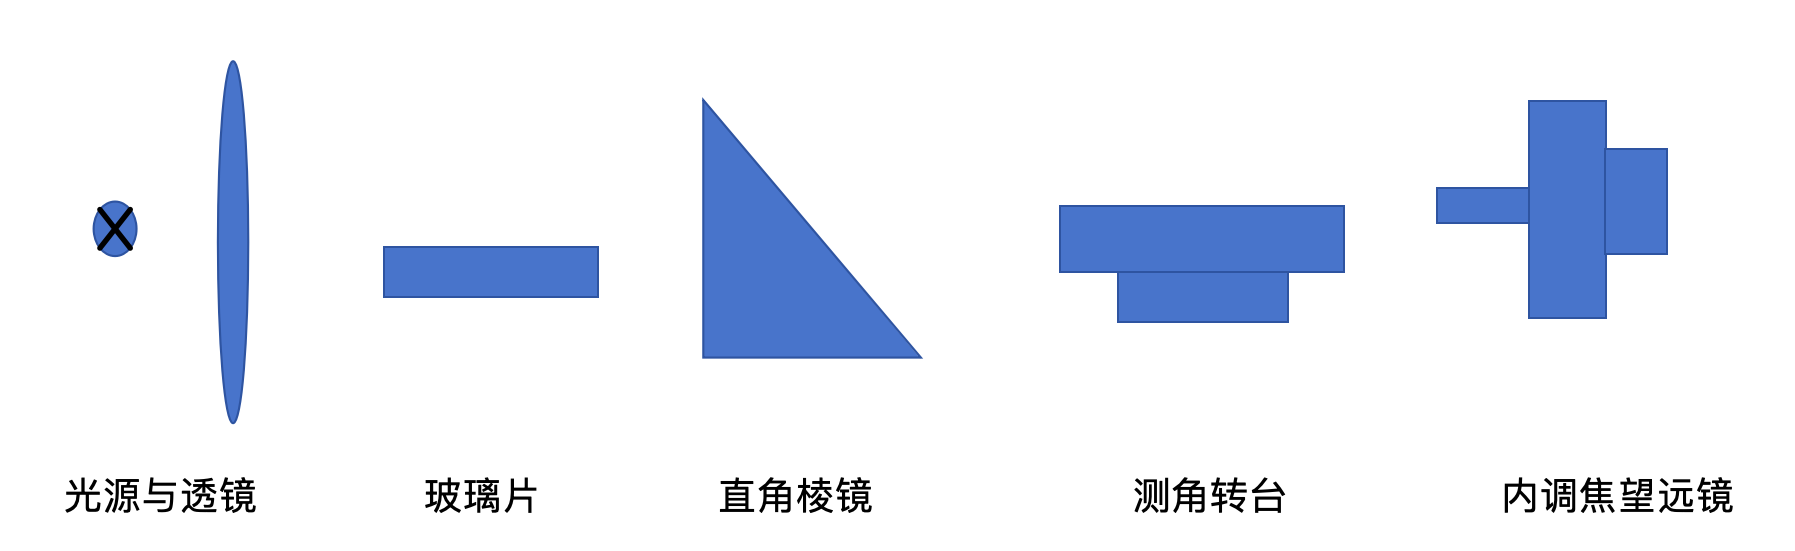
\includegraphics[width=0.7\linewidth]{131.png}
                
        \end{figure}

\end{enumerate}
\end{document}